\documentclass[11pt,class=article,float=false,crop=false]{standalone}
%\documentclass[11pt]{article}
\usepackage{Part3_packages}

\begin{document}

\section{Gestion des collisions}

La gestion des collisions consiste à déplacer et fusionner les lignes de dislocation en fonction des contacts qui ont lieu. Il faut effectuer dans l'ordre toutes les collisions qui ont été détectées à l'étape précédente. De nouvelles collisions non détectées précédemment pourront être induites par la modification du réseau, il faut donc effectuer une détection partielle à chaque modification pour ne pas courir le risque de rater des collisions. Le nombre de collisions ayant lieu au cours d'un pas de temps est normalement faible par rapport au nombre de dislocations. La performance n'est pas cruciale pour cette étape, mais il faudra tout de même faire attention à ne pas faire exploser la complexité de la mise à jour des collisions. 

Dans cette partie, nous verrons en premier lieu quelles sont les modifications topologiques à effectuer lors d'une collision entre deux objets. Nous verrons ensuite comment effectuer ces opérations dans l'ordre en prenant en compte toutes les collisions.

\subsection{Opérations topologiques}

\label{sec:operations_topologiques}

Cette partie détaille les modifications topologique à effectuer pour chaque type de collision rencontrée. Ces opérations topologiques sont aussi décrites dans le livre de V. Bulatov et al. (10.4) \citecol{bulatov2006computer}.

\subsubsection{Données portées par les segments}

En dynamique des dislocations, chaque segment porte des propriétés physiques. Pour modifier la topologie du réseau, les propriétés qui nous intéressent en plus des propriétés géométriques sont celle liées au système de glissement. Chaque segment se déplace dans un plan de glissement et est caractérisé par un vecteur de Burgers. Il est important que chaque modification géométrique respecte ces propriétés physiques : Les déplacements doivent se faire dans les plans de glissement des segments et les données portées par les nouveaux segments insérés doivent être cohérentes.


\subsubsection{Point/Point}

Lorsque deux points entrent en collision, ces deux points fusionnent, formant un unique point dont la vitesse est la moyenne des vitesses des points fusionnés, comme le montre la figure \ref{fig:topo_pointpoint}. 

\begin{figure}[H]
	\centering
	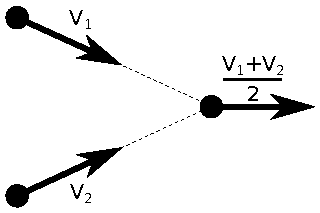
\includegraphics[height=0.15\textheight]{img/topo_pointpoint}
	\caption{Collision de deux nœuds.}
	\label{fig:topo_pointpoint}
\end{figure}

Les segments précédemment connectés aux deux nœuds fusionnés sont transférés au nouveau nœud. Dans le cas particulier illustré dans la figure \ref{fig:topo_fusionsegments}, les nœuds qui entrent en collision sont connectés au même nœud. Après la collision, le segment double doit être fusionné en un unique segment dont les propriétés sont les suivantes:
\begin{itemize}	
	\item Vecteur de Burgers : Sommation de Burgers \footnote{Attention au sens de parcours de la dislocation}. Si vecteur de Burgers résultant est nul, le nouveau segment doit être supprimé;
	\item Plan de glissement : Doit être celui formé par le vecteur directeur et le vecteur de Burgers \footnote{Dans le cas particulier de la dislocation vis, le système de glissement le plus favorable est choisi }. 
\end{itemize}

\begin{figure}[H]
	\centering
	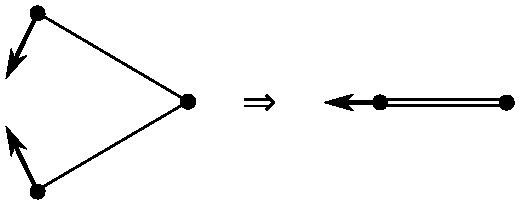
\includegraphics[height=0.15\textheight]{img/topo_fusionsegments}
	\caption{Fusion d'un segment.}
	\label{fig:topo_fusionsegments}
\end{figure}

Pour que le résultat soit en accord avec la physique des dislocations, il ne faut pas oublier de projeter la vitesse sur les plans de glissement de tous les segments connectés au nœud nouvellement crée. De cette manière, chaque segment se déplace bien dans son plan de glissement. De plus, il faut s'assurer que le nouveau segment est bien inclu dans l'intersection des plans de glissement des segments fusionnés.

\subsubsection{Point/Segment}

Lorsqu'un point entre en collision avec un segment loin des bords de celui-ci, le point est fusionné avec le segment comme l'illustre la figure \ref{fig:topo_pointseg}. Comme précédemment, il faut fusionner les segments dupliqués et projeter les vitesses sur les plans de glissement.

\begin{figure}[H]
	\centering
	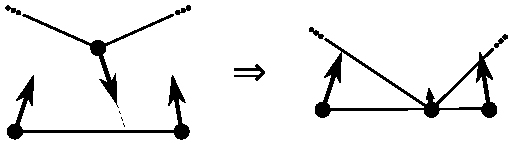
\includegraphics[height=0.15\textheight]{img/topo_pointseg}
	\caption{Collision d'un nœud avec un segment.}
	\label{fig:topo_pointseg}
\end{figure}

\paragraph{Vitesse du point de collision}
\label{sec:dents_de_scie}

La vitesse du nœud fusionné avec le segment doit être déterminée en fonction des vitesses des objets qui entrent en collision. L'idée la plus simple consiste à prendre comme nouvelle vitesse la moyenne entre la vitesse du nœud $n_3$ et la vitesse du segment au point de collision:

\begin{equation}
	v_3^\prime = \frac{(\alpha v_1 + (1-\alpha)v_2) + v_3 }2
\end{equation}

avec $\alpha \in [0,1]$ le paramètre de la position du point de collision sur le segment $S = [1-2]$.

Cette solution simple pose un problème car elle dépend de l'ordre des collisions. Dans l'exemple de la figure \ref{fig:vitesse_pointseg_probleme}, deux lignes de dislocations entrent en contact. Dans cet exemple, tous les nœuds entrent en contact au même moment avec les segments donc il faut choisir un ordre pour gérer ces collisions. Selon l'ordre choisi le résultat est différent. Par exemple dans la figure, on fusionne les nœuds de la ligne du bas en premier : deux nœuds de la ligne ont une vitesse non nulle. Si on avait fusionné la ligne du haut en premier, les nœuds encore mobiles ne seraient pas les mêmes.

\begin{figure}[H]
	\centering
	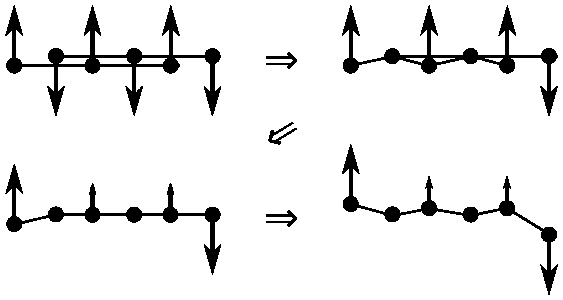
\includegraphics[height=0.3\textheight]{img/vitesse_pointseg_probleme}
	\caption{Collision de deux lignes de dislocation.}
	\label{fig:vitesse_pointseg_probleme}
\end{figure}

Une solution à ce problème est d'utiliser toujours les mêmes valeurs pour $v_1$ et $v_2$ au cours du pas de temps. On peut par exemple utiliser la valeur de la vitesse au début du pas de temps. De cette manière, l'effet dents-de-scie est atténué. 


\subsubsection{Segment/Segment}

Pour le cas de la collision entre deux segments, il ne reste plus qu'a traiter le cas ou les deux segments ne se trouvent pas dans le même plan. En effet, si deux segments d'un même plan entrent en collision, le contact se fera nécessairement par une des extrémités d'un des deux segments : il s'agit alors d'une collision Point/Segment ou Point/Point. Les deux segments entrent donc en contact en un unique point. 

Deux points sont crées sur les 2 segments au niveau du point de collision, puis sont fusionnés comme le montre la figure \ref{fig:topo_segseg}.

\begin{figure}[H]
	\centering
	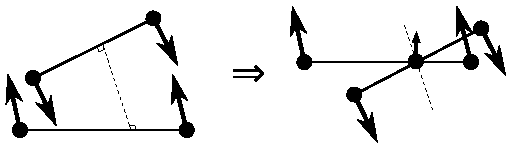
\includegraphics[height=0.15\textheight]{img/topo_segseg}
	\caption{Collision de 2 segments en 3 dimensions.}
	\label{fig:topo_segseg}
\end{figure}

La vitesse du nouveau point est la moyenne des vitesses des points de collision sur chaque segment. La symétrie des objets (Segment/Segment) assure qu'il n'y a pas de problèmes de dissymétrie comme pour Point/Segment. Comme le nouveau nœud n'est connecté qu'aux extrémités des segments, il n'y a pas de problème de fusion des segments. 

\subsection{Algorithmes de gestion des collisions}

Les différents algorithmes de gestion des collisions étudiés sont décrit dans cette section. Un algorithme en particulier a été choisi pour être intégré dans OptiDis. Les raisons de ce choix, ainsi que son implémentation précise seront détaillés dans cette section.

\subsubsection{Fusion de proximité}

Le premier algorithme étudié utilise une détection statique des collisions pour fusionner les objets proches. Il s'agit d'une variante de l'algorithme évoqué dans \citecol{sills2016advanced} qui limite le pas de temps à $dt < 2r_{col}/v_{max}$. Si le pas de temps est plus grand que la limite évoquée précédemment, il est possible de découper le pas de temps $dt$ en sous pas de temps $dt_{col}$ tel que $dt_{col} <2r_{col}/v_{max}$. L'algorithme effectue des sous pas de temps successifs en alternant une détection de collisions statique, et une fusion de proximité et déplaçant à chaque sous pas de temps les dislocations. Le diagramme \ref{fig:algo_collision_statique} illustre cet algorithme.

\begin{figure}[H]
	\centering
	\includetikz{img/algo_collision_statique}
	\caption{Algorithme de collision : Fusion de proximité.}
	\label{fig:algo_collision_statique}
\end{figure}

Cet algorithme a pour avantage d'être facile à implémenter et robuste, ce qui en fait un bon algorithme de référence pour vérifier la validité des autres algorithmes. Cependant, même en utilisant une méthode d'intégration explicite, un grand nombre de sous pas de temps est nécessaire. Les pas de temps $dt$ utilisés pour un intégrateur \textit{forward euler} sont de l'ordre de $dt \approx L/v_{max}$ avec $L$ de l'ordre de grandeur de la longueur d'un segment. $L$ est grand devant $r_{col}$, donc le nombre de sous-pas de temps à effectuer est important.

\subsubsection{Gestion de collision séquentielle}

L'algorithme de gestion séquentiel des collisions commence après une phase de détection dynamique complète. Les collisions détectées sont stockées dans une liste globale de collisions. L'algorithme parcourt les collisions dans l'ordre chronologique. Pour chaque collision détectée au temps $t_{col}$ entre les objets $o_1$ et $o_2$, l'ensemble du réseau de dislocations est déplacé au temps $t_{col}$, puis l'opération topologique de la fusion entre $o_1$ et $o_2$ est effectuée. La modification du réseau peut engendrer de nouvelles collisions : une re-détection de collision doit être effectuée pour les objets qui ont été modifiés. Cette opération est moins coûteuse qu'une détection globale. Le diagramme de la figure \ref{fig:algo_collision_sequentiel} illustre le déroulement de cet algorithme.

\begin{figure}[H]
	\centering
	\includetikz{img/algo_collision_sequentiel}
	\caption{Algorithme de collision : séquentiel.}
	\label{fig:algo_collision_sequentiel}
\end{figure}

Cet algorithme possède une complexité moins importante que l'algorithme à fusion de proximité, et reste relativement facile à mettre en œuvre. Afin d'obtenir les meilleures performances pour cet algorithme, des optimisations sont possibles. Le déplacement des dislocations et le re-calcul des collisions sont les opérations les plus coûteuses de l'algorithme et peuvent être optimisées. 

Le re-calcul des collisions pour les objets qui ont été modifiés au cours des modifications topologiques peut utiliser les mêmes techniques que pour la détection globale des collisions. Le découpage en grille uniforme permet de ne tester que les dislocations des boites voisines des objets modifiés. 

L'optimisation du déplacement des dislocations fait l'objet de la section suivante.

\subsubsection{Gestion de collision séquentielle sans déplacement}
\label{sec:operations_topologiques_nomove}

Le déplacement des nœuds du réseau de dislocations dans l'algorithme \ref{fig:algo_collision_sequentiel} est linéaire en nombre de dislocations. Il est possible d'éviter cette étape en modifiant les opérations topologiques pour n'avoir à déplacer les dislocations qu'une seule fois à la fin de l'algorithme. Pour cela, les opérations topologiques doivent être modifiées pour prendre en compte que les objets ne sont pas proches au moment d'effectuer l'opération topologique. Les opérations sont modifiées de la manière suivante:

\paragraph{Point/Point}

Lorsque deux nœuds du réseau de dislocations entrent en collision, ils fusionnent pour former un unique point, comme le montre la figure \ref{fig:collision_pointpoint}.

\begin{figure}[h]
	\centering
	\includetikz{img/topo_nomove_pointpoint}
	\caption{Fusion de deux nœuds du réseau de dislocations.}
	\label{fig:collision_pointpoint}
\end{figure}

Le nouveau nœud est placé où à lieu la collision, c'est à dire à la position que prennent $n_1$ et $n_2$ au temps de collision $t_{col}$:
\begin{equation}
\begin{split}
n_{new} & = n_1 + t_{col} \cdot v_1 \\
& = n_2 + t_{col} \cdot v_2
\end{split}
\end{equation}

La nouvelle vitesse est calculée pour que le nœud soit positionné à la fin du pas de temps ($t=dt$) comme s'il s'était déplacé à la vitesse $\frac{v_1+v_2}2$ pendant le reste du pas de temps. Cela permet de compenser le déplacement déjà effectué:
\begin{equation}
v_{new} = \frac{v_1+v_2}2 \frac{dt-t_{col}}{dt}
\end{equation}

\paragraph{Point/Segment}

Lors de la collision entre un nœud et un segment, le nœud qui entre en collision est fusionné avec le segment, comme le montre la figure \ref{fig:topo_nomove_pointseg}.

\begin{figure}[h]
	\centering
	\begin{subfigure}[b]{0.5\textwidth}
		\centering
		\includetikz{img/topo_nomove_pointseg_initial}
		\caption{État initial du réseau.}
		%\label{fig:topo_pointseg_initial}
	\end{subfigure}%
	\begin{subfigure}[b]{0.5\textwidth}
		\centering
		\includetikz{img/topo_nomove_pointseg_fused}
		\caption{Réseau après l'opération topologique.}
		%\label{fig:topo_pointseg_fused}
	\end{subfigure}
	\caption{Opération topologique effectuée lors de la collision d'un nœud avec un segment.}
	\label{fig:topo_nomove_pointseg}
\end{figure}

Seul le point $n_3$ est modifié pour se transformer en $n_{new}$ : les autres nœuds du réseau restent inchangés. La topologie du réseau est modifiée en remplaçant le segment $(n_1,n_2)$ par les segments $(n_1,n_{new})$ et $(n_2,n_{new})$.

Le nouveau nœud est placé où à lieu la collision:
\begin{equation}
n_{new} = n_3 + t_{col} \cdot v_3
\end{equation}

La vitesse du nouveau point doit s'apparenter à la moyenne entre la vitesse $v_3$ du nœud $n_3$ et la vitesse $v_{12}$ du point de collision sur le segment $(n_1,n_2)$. Comme auparavant, la vitesse est ajustée pour compenser le déplacement déjà effectué:

\begin{equation}
v_{new} = \frac{v_3+v_{12}}2 \frac{dt-t_{col}}{dt}
\end{equation}

$v_{12}$ peut être calculée en déplacent le segment $(n_1,n_2)$ au temps de collision et en effectuant un calcul de barycentre:

\begin{equation}
\begin{split}
v_{12} = & \frac{||n_1(t_{col})n_{new}|| \cdot v_1 + ||n_2(t_{col})n_{new}|| \cdot v_2}
{||n_1(t_{col})n_2(t_{col})||} \\                
\text{avec } & n_i(t) = n_i + t \cdot v_i
\end{split}
\end{equation}

Si $n_1$ est $n_2$ ont déjà été modifiés par d'autres opérations topologiques auparavant, il est préférable (si possible) d'utiliser les vitesses que ces nœuds avaient initialement afin d'éviter la formation de dents de scie\footnote{Voir section \ref{sec:dents_de_scie}}.

\paragraph{Segment/Segment}

Lors de la collision entre deux segments, les deux segments sont fusionnés en un point à l'endroit où a lieu la collision, comme le montre la figure \ref{fig:topo_nomove_segseg}.

\begin{figure}[h]
	\centering
	\begin{subfigure}[b]{0.5\textwidth}
		\centering
		\includetikz{img/topo_nomove_segseg_initial}
		\caption{État initial du réseau.}
		%\label{fig:topo_segseg_initial}
	\end{subfigure}%
	\begin{subfigure}[b]{0.5\textwidth}
		\centering
		\includetikz{img/topo_nomove_segseg_final}
		\caption{Réseau après l'opération topologique.}
		%\label{fig:topo_segseg_final}
	\end{subfigure}
	\caption{Opération topologique effectuée lors de la collision entre deux segments.}
	\label{fig:topo_nomove_segseg}
\end{figure}

Les nœuds existants préalablement ne se déplacent pas, mais la  topologie du réseau et modifiée en remplaçant le segment $(n_1,n_2)$ par les segments $(n_1,n_{new})$ et $(n_2,n_{new})$ , et le segment $(n_3,n_4)$ par $(n_3,n_{new})$ et $(n_4,n_{new})$.

Le nouveau nœud est placé où a lieu la collision. Pour déterminer le lieu de la collision, il faut calculer les paramètres sur les droites du lieu de collision. Les nœuds sont déplacés au temps de la collision, et la formule inspirée de \citecol{bourkeshortest} est utilisée :

\begin{equation}
\begin{split}
a_{12} &= \frac{ (\vec{31} \cdot \vec{34})(\vec{34} \cdot \vec{12}) - (\vec{31} \cdot \vec{12})(\vec{34} \cdot \vec{34}) }
{ (\vec{21} \cdot \vec{21})(\vec{34} \cdot \vec{34}) - (\vec{34} \cdot \vec{12})(\vec{34} \cdot \vec{12}) } \\
a_{34} &= \frac{ (\vec{31} \cdot \vec{34}) + (\vec{34} \cdot \vec{21}) \cdot a_{12} }{||\vec{34}||^2}
\end{split}
\end{equation}

On obtient la position de collision par la formule suivante:

\begin{equation}
\begin{split}
n_{new} &= a_{12} \cdot n_1(t) + (1-a_{12}) \cdot n_2(t) \\
&= a_{34} \cdot n_3(t) + (1-a_{34}) \cdot n_4(t)
\end{split}
\end{equation}

La vitesse du nouveau point est la moyenne des vitesses des points de collision sur les segments. Cette vitesse est ajustée pour compenser le mouvement déjà effectué:

\begin{equation}
v_{new} = \frac{v_{12}+v_{34}}2 \frac{dt-t_{col}}{dt}
\end{equation}

$v_{12}$ et $v_{34}$ sont calculées en calculant le barycentre en utilisant les paramètres $a_{12}$ et $a_{34}$:

\begin{equation}
v_{ij} = a_{ij} v_i + (1-a_{ij}) v_j
\end{equation}


\subsubsection{Algorithme de gestion parallèle des collisions.}

Intuitivement, lorsque deux collisions sont \textit{suffisamment lointaines} le traitement d'une collision n'influe pas sur la deuxième et il est possible de traiter les deux collisions parallèlement. La notion de collisions \textit{suffisamment lointaines} s'appuie en fait sur un ordre partiel dans lequel les collisions doivent être traitées. En contraste avec l'algorithme séquentiel qui utilise un ordre total, un algorithme parallèle doit pouvoir gérer plusieurs collisions en même temps. 

Définir un ordre partiel sur les collisions revient à définir la relation $<$ telle que pour une collision $c$, l'ensemble $\{c_i | c_i < c \}$ soit l'ensemble des collisions qui doivent être traitées avant la collision $c$. Par exemple la relation d'ordre utilisée pour les algorithmes séquentiels est l'ordre chronologique:

\begin{equation}
	 c_1 <_{seq} c_2 \Leftrightarrow c_1.t_{col} < c_2.t_{col}
\end{equation}

Cette condition est sur-contrainte pour obtenir un ordre total qu'il est possible de parcourir séquentiellement. Une collision $c_1$ doit être traitée avant $c_2$ si $c_1$ modifie des objets impliqués dans $c_2$ avant que la collision $c_2$ ait lieu. Soient $M_c$ les objets modifiés par $c$ et $O_c$ les objets qui entrent en collision pendant la collision $c$. D'ou la relation $<_{parallel}$ utilisable pour un algorithme parallèle:

\begin{equation}
c_1 <_{parallel} c_2 \Leftarrow c_1.t_{col} < c_2.t_{col} \wedge M_{c_1} \cap O_{c_2} = \emptyset
\end{equation}

\paragraph{}
L'algorithme de traitement parallèle proposé utilise un modèle à agents. Chaque segment de dislocation possède son comportement qui lui est propre. Pour chaque segment, on connait l'ensemble  $C_s$ des collisions dans lesquelles il intervient. Le segment parcoure l'ensemble de ses collisions dans l'ordre chronologique. Avant de traiter une collision, le segment doit s'assurer que la collision est minimale selon $<_{parallel}$. C'est à dire qu'il n'existe pas de collision devant être gérée antérieurement à celle en cours de traitement. Le segment met en attente le traitement de la collision jusqu'à ce que les autres segments aient traités les collisions antérieures. Lorsque le \textit{test de précédence} vérifie qu'aucune collision n'est antérieure, le segment peut traiter sa collision. La figure \ref{fig:collision_algo_parallele} résume l'algorithme parallèle de gestion des collisions exécuté en parallèle pour chaque segment.

\begin{figure}[h]
	\centering
	\includetikz{img/collision_algo_parallele}
	\caption{L'algorithme parallèle de gestion des collisions.}
	\label{fig:collision_algo_parallele}
\end{figure}

Le \textit{test de précédence} parcoure les listes de collisions de tous les éléments $o \in M_c$ et vérifie si leur liste de collisions $C_o$ contient une collision chronologiquement antérieure. Tant qu'une telle collision existe, le traitement est mis en attente.

\paragraph{}
La gestion parallèle des collisions pose plusieurs problèmes. Premièrement, l'accès à la structure de données contenant les dislocations pour modifier la topologie doit se faire de manière concurrente. Le code de démonstration ne proposant pas d'accès parallèle à cette structure, les modifications topologiques sont séquentialisées. Ensuite, le grain de parallélisme proposé dans cet algorithme est trop fin : traiter chaque segment dans un thread différent n'est pas possible. Pour grossir le grain de parallélisme, il est possible de grouper de segments. Une gestion réellement parallèle des collisions est difficile à mettre en place, et nous verrons qu'elle n'est pas forcément nécessaire.

\end{document}